\documentclass{beamer}
\usepackage[utf8]{inputenc}
\usepackage[brazil]{babel}
\usepackage{subfigure}
\usetheme{Malmoe}

\title[Universidade Católica do Salvador]{Extração de Informações de Dependência entre Módulos de Programas C/C++}
\author[Joenio Costa]{Joenio Marques da Costa}
\institute{UCSal - Universidade Católica do Salvador}
\date{13 junho de 2009}
\subject{alguma coisa}
\logo{
\includegraphics[scale=0.15]{imagens/brasao-ucsal-pb}}

\begin{document}

\frame{\titlepage} %para criar a página de rosto

\begin{frame}
 \tableofcontents
\end{frame}

\section{Objetivo}

\begin{frame}
\frametitle{Objetivo}
 Implementar uma ferramenta para extração de informações de dependências
 entre módulos de programas escritos em C/C++ sem necessidade de compilação.
\end{frame}

\section{Conceitos}

\subsection{Arquitetura de Software}

\begin{frame}
\frametitle{Arquitetura de Software}
 Arquitetura de software de um programa é a estrutura que define as propriedades
 externamente visíveis e o relacionamento entre os grandes componentes
 estruturais de um sistema.
\end{frame}

\subsection{Coesão e Acoplamento}

\begin{frame}
\frametitle{Coesão e Acoplamento}
\framesubtitle{atributos de modularidade}
 \begin{description}
 \item[Coesão]É a medida que define o quanto um módulo de um programa está
 focado em solucionar um único problema. Quanto maior a coesão menor o
 acoplamento
 \item[Acoplamento]Representa o nível de interdependências entre os módulos de
 um sistema. Quanto maior o acoplamento maior a complexidade.
 \end{description}
\end{frame}

\subsection{Métricas}

\begin{frame}
\frametitle{Métricas}
\framesubtitle{coesão e acoplamento}
 \begin{description}
 \item[LCOM] Falta de coesão em métodos\newline (lack of cohesion in methods)
 \item[CBO] Acoplamento entre as classes de objetos\newline (coupling between objects classes)
 \end{description}
\end{frame}

\section{Implementação do Extrator}

\subsection{egypt}

\begin{frame}
\frametitle{egypt\footnote{http://www.gson.org/egypt}}
 O egypt é um Software Livre desenvolvido com o objetivo de gerar grafos de
 chamada entre funções de programas escritos em C/C++.
 \begin{figure}[h]
 \center
 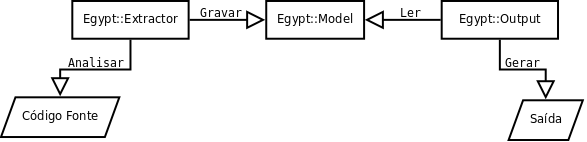
\includegraphics[scale=0.3]{imagens/egypt-fluxogram}
 \label{fig:egypt-fluxogram}
 \end{figure}
\end{frame}

\subsection{Doxygen}

\begin{frame}
\frametitle{Doxygen\footnote{http://www.doxygen.org}}
\framesubtitle{sistema de documentação}
 Possui um parser para cada linguagem suportada.
 \begin{figure}[h]
 \center
 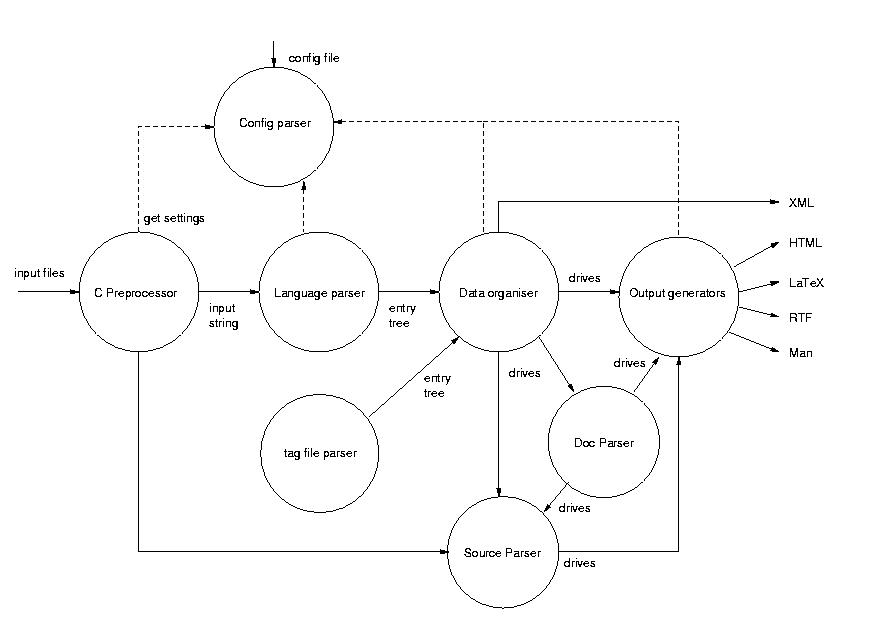
\includegraphics[scale=0.25]{imagens/doxygen-internals-flow}
 \label{fig:doxygen-internals-flow}
 \end{figure}
\end{frame}

\subsection{egypt + Doxygen}

\begin{frame}
\frametitle{egypt + Doxygen}
\framesubtitle{doxyparse\footnote{http://gitorious.org/projects/doxygen}}
 Um parser capaz de analisar projetos escritos em C/C++ e identificar onde os
 símbolos são declarados e utilizados dentro do do projeto.
 \begin{figure}[h]
 \center
 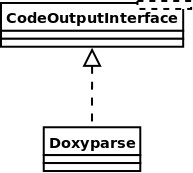
\includegraphics[scale=0.3]{imagens/doxyparse-diagram}
 \label{doxyparse-diagram}
 \end{figure}
\end{frame}

\begin{frame}
\frametitle{egypt + Doxygen}
\framesubtitle{Egypt::Exractor::Doxyparse\footnote{http://github.com/terceiro/egypt}}
 Um extrator para o egypt baseado no doxyparse.
 \begin{figure}[h]
 \center
 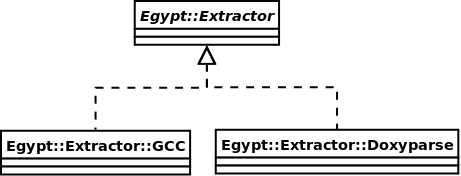
\includegraphics[scale=0.3]{imagens/egypt-diagram-extractor}
 \label{egypt-diagram-extractor}
 \end{figure}
\end{frame}

\section{Avaliação}

\subsection{Procedimento}

\begin{frame}
\frametitle{Procedimento}
\framesubtitle{caso de uso ristretto}
\begin{itemize}
 \item ristretto é um Software Livre escrito em C para visualização de imagens no
 ambiente Desktop Xfce\footnote{http://www.xfce.org}.
 \item 21 versões do projeto foram analisadas utilizando o novo extrator do egypt,
 os resultados foram comparados aos dados obtidos pelo extrator original.
\end{itemize}
\end{frame}

\subsection{Resultados}

\begin{frame}
\frametitle{Resultados}
\framesubtitle{grafo do ristretto 0.0.11}
 \begin{figure}
 \center
 \subfigure[Doxyparse]{
  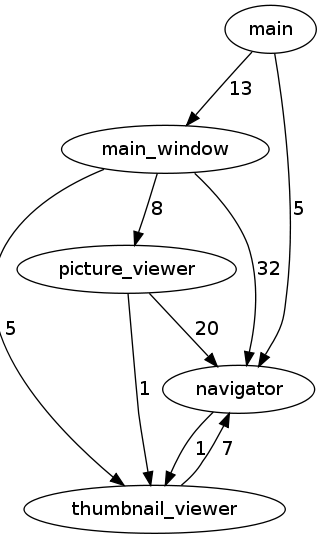
\includegraphics[scale=0.25]{imagens/ristretto-0_0_11-doxyparse}
  \label{fig:ristretto-0.0.11-doxyparse}
 }
 \qquad
 \subfigure[GCC]{
    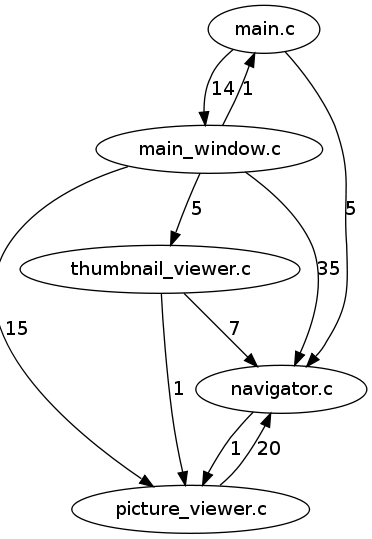
\includegraphics[scale=0.25]{imagens/ristretto-0_0_11-gcc}
    \label{fig:ristretto-0.0.11-gcc}
 }
 \label{fig:ristretto-0.0.11}
 \end{figure}
\end{frame}

\begin{frame}
\frametitle{Resultados}
\framesubtitle{o que são essas diferenças}
 \begin{itemize}
 \item egypt confunde o uso de símbolos com mesmo nome
 \item doxyparse não avalia bem os símbolos estáticos
 \item egypt erra o cálculo de CBO (acoplamento)
 \end{itemize}
\end{frame}

\begin{frame}
\frametitle{Resultados}
\framesubtitle{grafo do ristretto 0.0.11 atualizado}
 \begin{figure}
 \center
 \subfigure[Doxyparse antes]{
    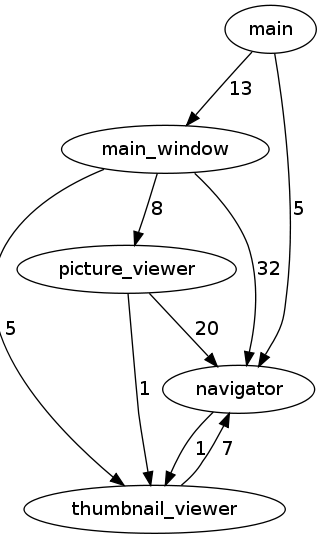
\includegraphics[scale=0.25]{imagens/ristretto-0_0_11-doxyparse}
 }
 \qquad
 \subfigure[Doxyparse depois]{
    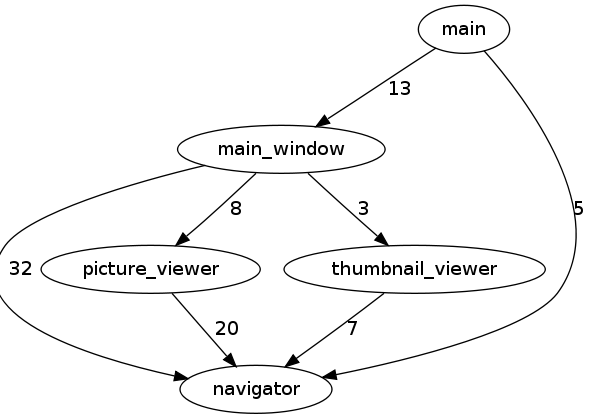
\includegraphics[scale=0.25]{imagens/ristretto-0_0_11-doxyparse-2}
 }
 \label{fig:ristretto-0.0.11-antes-depois}
 \end{figure}
\end{frame}

\section{Conclusão}

\begin{frame}
\frametitle{Conclusão}
 O objetivo inicial foi atingido, implementar uma ferramenta para extração de
 informação de dependência entre módulos de programas escritos em C/C++.
\end{frame}

\subsection{Trabalhos futuros}

\begin{frame}
\frametitle{Trabalhos futuros}
 \begin{itemize}
 \item Testar egypt em outras linguagens de programação
 \item Implementar novo extrator baseado em Natural Docs\footnote{http://www.naturaldocs.org}
 \item Implementar no doxyparse detecção de chamada indireta
 \item Armazenar símbolos externos ao projeto
 \end{itemize}
\end{frame}

\end{document}
